\documentclass[12pt,a4paper]{article}
\usepackage[utf8]{inputenc}
\usepackage{graphicx}
\usepackage[frenchb]{babel}

\title{Snake}
\author{Antoine Forgerou \and Jérémy Bardon}
\date{}

\begin{document}

\maketitle
\vspace{0.80cm}
\begin{abstract}
    Dans le cadre du module de logiciel extensible, nous avons développez une plateforme permettant de charger des plugins de manière reflexive. Pour illustrer le fonctionnement de cette plateforme, nous avons recréé le célèbre jeu du snake.
\end{abstract} 
\vspace{0.80cm}
\tableofcontents

\newpage

   
    
\section{Introduction}

    Dans le cadre de notre projet, l'interet de développer le jeu du snake est double. Le premier avantage est que le jeu est assez simple à coder, nous permettant de nous concentrer sur la partie "plugins" du projet et non sur le développement du snake en lui-meme. Le second est que la plupart des composants du jeu peuvent être des plugins (affichage, map, score, etc ...).\\
    
\section{Plugin Principal}    
    
    L'application est donc séparée en multiple plugins. Le coeur de l'application est le plugin principale (runnable par la plateforme) appelé \textbf{snakecore}. Ce plugin est unique et gère le fonctionnement principale du snake. Pour fonctionner, il utilise des plugins secondaires respectant les besoins qu'il leurs impose à travers des interfaces.\\

    Lors du lancement le plugin lance une interface permettant soit de lancer le jeu, soit de lancer une interface de configuration permettant de choisir les plugins utilisées. Des plugins sont choisies par défaut permettant de jouer directement. \\

\begin{figure}[h]
    \centering
    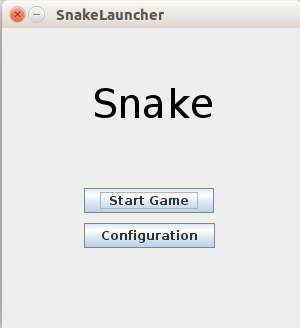
\includegraphics[scale=0.5]{ressourcesSnake/menu.png}
    \caption{Menu du Snake}
\end{figure}    

\newpage
    Dans l'interface de configuration des plugins, les plugins sont triés par type. Pour chaque type, la liste des plugins disponibles est affichés ainsi que le nombre séléctionnable.\\

\begin{figure}[h]
    \centering
    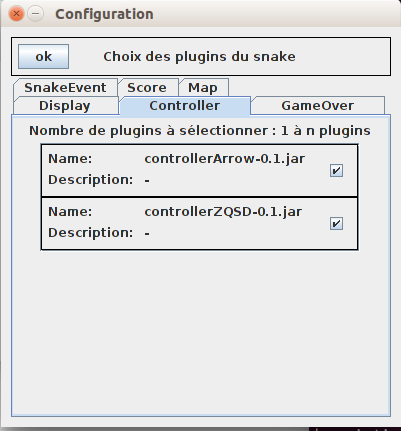
\includegraphics[scale=0.4]{ressourcesSnake/configurationControler.png}
    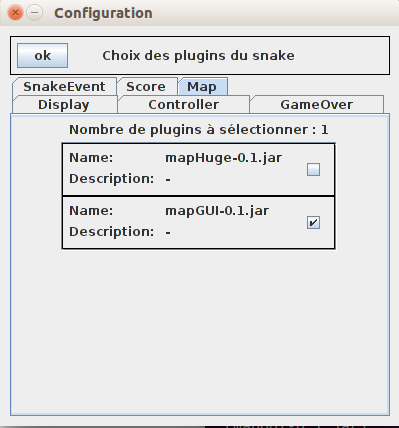
\includegraphics[scale=0.4]{ressourcesSnake/configurationMap.png}
    \caption{interface de configuration - Controler / Map}
\end{figure}       
    
    Quand le jeu est lancé, le plugin principal demande à la plateforme de charger la liste des plugins séléctionnés afin de pouvoir les utilisées. Une fois les plugins secondaires chargés, le moteur du snake est lancé jusqu'à la défaite du joueur. \\

\begin{figure}[h]
    \centering
    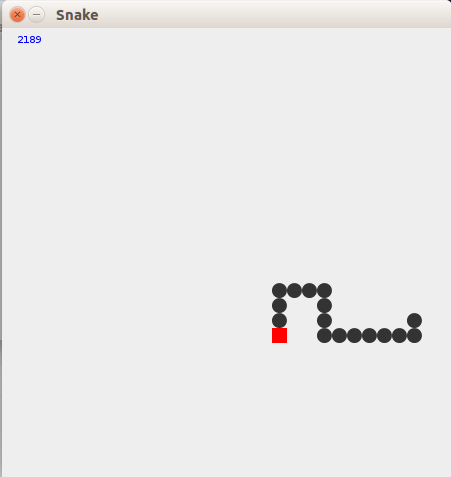
\includegraphics[scale=0.4]{ressourcesSnake/snake.png}
    \caption{Une partie de Snake}
\end{figure}   
    
\section{Plugins Secondaires}    
    
    L'interet de ce projet est de séparer chaques fonctionnalités en plugin. Le plugin principal défini les interfaces dont il a besoin ou qu'il supporte. Les plugins secondaires peuvent être classées en plusieurs catégories. En effet certains plugins sont essentiels au bon fonctionnement du programme alors que d'autres sont optionnels. Deplus certains plugins peuvent être multiples pour une même catégorie alors que d'autres sont uniques. 
    
    \subsection{ L'interface}
    
    L'interface d'affichage que va utiliser le plugin principal est un plugin. En effet, il est possible d'imaginer plusieurs interfaces graphiques différentes. Ce type de plugin est nécessaire au fonctionnement du programme. Deplus, il est unique car nous souhaitons jouer avec une seule interface.
    
    \subsection{ La map}
    
    Ce type de plugin représente la map sur laquelle ce déplace le serpent. Le seule interet de ce plugin est de spécifié la taille de la map. On pourrait le considéré comme un plugin $"$data$"$ Ce plugin est aussi nécessaire pour l'application. Pour une partie donné, il ne peut y avoir qu'une map, ce type de plugin est donc unique.
    
    \subsection{ Controller le snake}
    
    Pour pouvoir jouer, il nécessaire de pouvoir changer la direction du snake. Ce controlleur peut être stocké dans un plugin. Le type Controlleur est nécessaire au bon fonctionnement, car il est impossibe de jouer sans. Nous avons choisi de permettre au joueur de pouvoir jouer avec plusieurs controlleurs simultanement, cette option n'entravant pas le bon fonctionnement du jeu.    
    
\newpage    
    \subsection{ Gestion du GameOver}
    
    Ce qui ce passe après la défaite du joueur (par défault contact avec lui même ou avec un mur) est géré par un type de plugin. Cependant, à travers ce plugin il est possible de modifier les conditions et les comportements de la défaite. Ce type de plugin est nécessaire pour pouvoir gérer la défaite du joueur.
    
    \subsection{ Un evenement particulier}
    
    Nous avons souhaitez pouvoir ajouter des comportements au cours de la partie. L'interet de ce plugin evenement est de pouvoir effectuer des actions à plusieurs moment de la partie. Ce type de plugin est optionnel mais peut aussi être multiple.\\
            Exemple : 
    \begin{itemize}
        \item Un plugin vitesse $\rightarrow$ augmente la vitesse de jeu à chaques tours.
        \item Un plugin evolution $\rightarrow$ modifie l'agrandissement du snake.    
    \end{itemize}
    
    
    

\end{document}
